\chapter{Generating binomial distributions}

\setcounter{problem}{1}
\section{Discussion}

\begin{fullwidth}

The goal of this lab is to simulate a binomial distribution using repeated Bernoulli trials and then compare it against the theoretical binomial distribution. Use filename {\tt rbinomial.py}.

\step First, set the seed of the random number generator. Otherwise you will always get the same  Bernoulli trials. In this case, we're using the current time in milliseconds as the random seed so that it is different every time you run the program. (remember this trick.)

\begin{pyverbatim}
np.random.seed( int(round(time.time() * 1000)) )
\end{pyverbatim}

\step Next, define a function that performs $n$ Bernoulli trials with probability $p$ of success. It should return the number of successes, $k$, out of $n$:

\begin{pyverbatim}
def binomial(n,p):
    "Sim with prob p, n bernoulli trials; return number of successes"
    ...
\end{pyverbatim}

The pseudocode is just a loop that goes around $n$ times and uses a variable from $U(0,1)$ to check for success or failure. For example, my solution assumes failure if the uniform random variable is greater than $p$.
    
\step Get list $X$ as $N$ Bernoulli trials with parameters $N=500$ and $P=0.4$. Do that by simply calling the {\tt bernoulli} function $N$ times.

\step Plot the histogram normalized (normed=1) and run it. you should see the following:

\scalebox{.35}{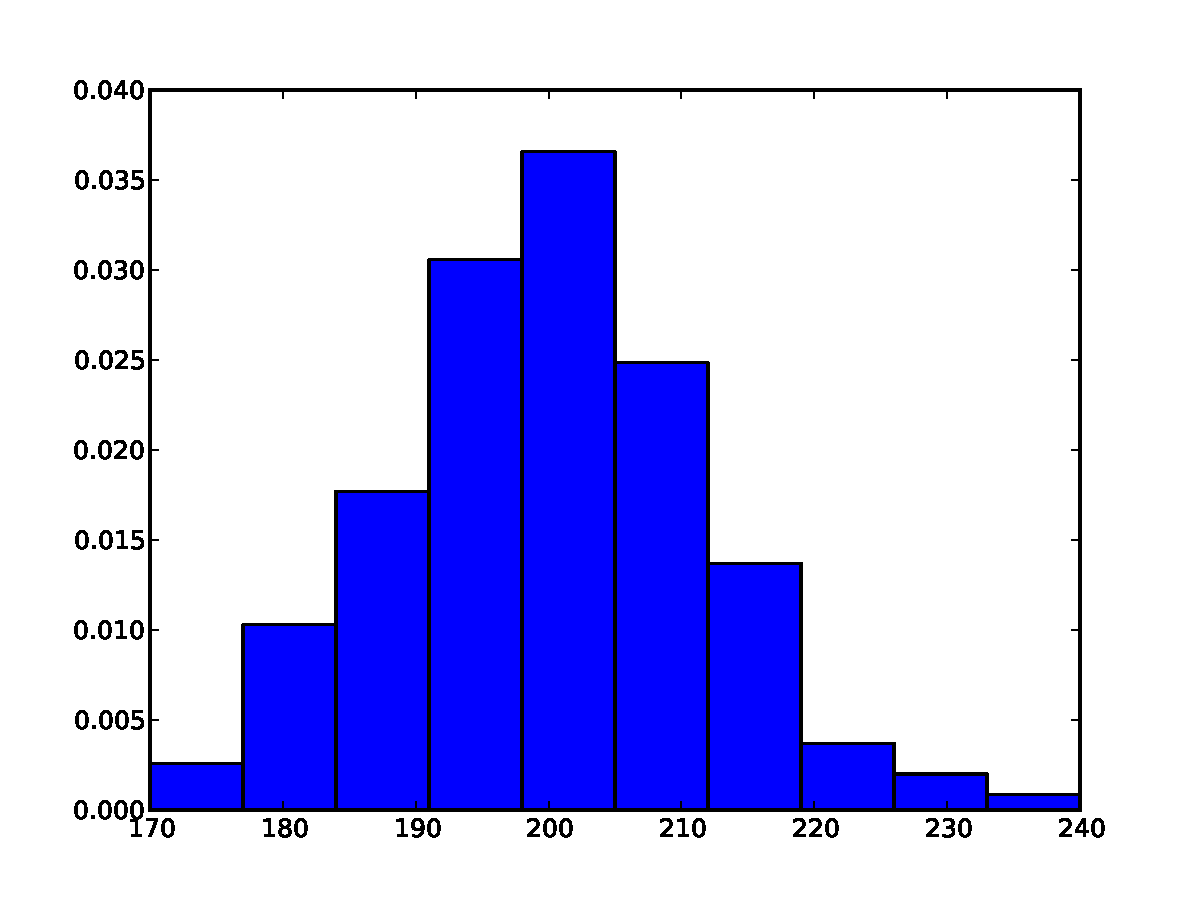
\includegraphics{figures/rbinomial-500-4.pdf}}

\step We could use the built-in binomial mass function but let's define our own since it's easy:

\[\tag{Binomial mass function}
\binom{n}{k} p^k (1-p)^{n-k}
\]

\noindent That's the probability that there are $k$ successes in $n$ trials with probability $p$ of success. Define a function like this:

\begin{pyverbatim}
def binom(k, n, p):
    """
    If we run n trials with p prob for each trial of success,
    how many have k successes?
    """
    ...
\end{pyverbatim}

\step To show the real distribution on top, we need to iterate $k$ across the range $0..N$ used in our empirical test above.  Since this is a mass function not a smooth density function, we can use every fifth value in the range. Let's also add some text to describe the parameters.

\begin{pyverbatim}
y = [binom(k, N, P) for k in range(0,N+1,5)]
plt.bar(range(0,N+1,5), y, color='red', align='center', width=1)
plt.axis([150,250,0,.05]) # set the axes so that we get a close-up
plt.text(160,0.04, '$N = %d$' % N, fontsize=16)
plt.text(160,0.037, '$P = %f$' % P, fontsize=16)
\end{pyverbatim}

In this case I am not using 0..1 for the axes coordinates of the text; the default is the values of the graph itself. sometimes this is useful.

\step Run it and you should see something like the following:

\scalebox{.35}{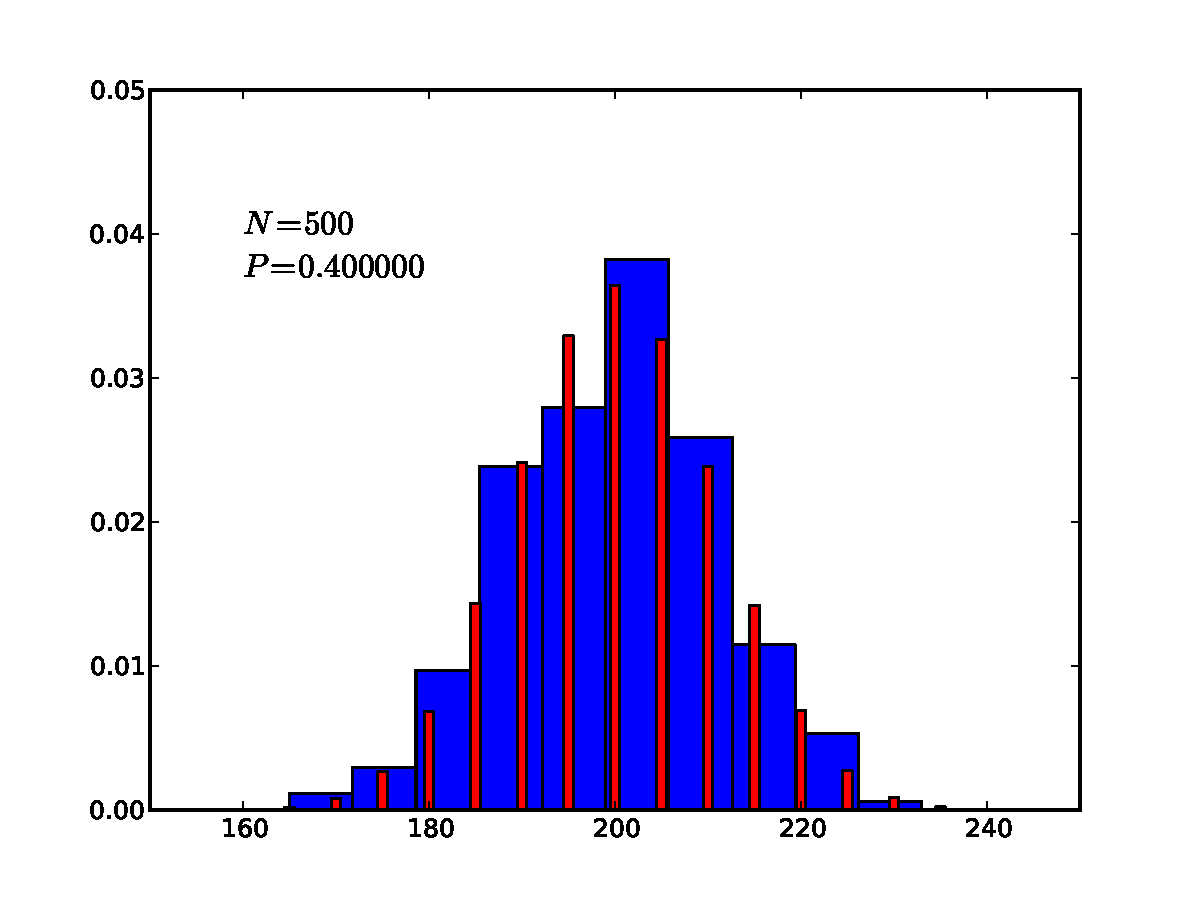
\includegraphics{figures/rbinomial-500-4-fancy.pdf}}

Note that we use a bar chart for the binomial theoretical distribution and not a smooth graph because this is a mass function not a density function.

\section{Deliverables}

Please submit:

\begin{itemize}
\item your Python file
\item submit a PDF of your final graph.
\end{itemize}

\end{fullwidth}
